\chapter{Исследовательская часть}

\section{Технические характеристики}

Технические характеристики устройства, на котором выполнялись замеры по времени, представлены далее:

\begin{itemize}
	\item Процессор -- 2 ГЦ 4‑ядерный процессор Intel Core i5;
	\item Оперативная память -- 16 ГБайт;
	\item Операционная система -- macOS Venura 13.5.2. 
\end{itemize}

\section{Пример работы}

В данном подразделе представлен пример \ref{lst:exmpl} работы программы: 

\begin{lstlisting}[label=lst:exmpl,caption=Пример работы программы]
    ivanmamvriyskiy@MacBook-Pro-Ivan-2 main % go run *.go
    1)Запустить конвейер
    2)Последовательная обработка
    3)Замер времени
    0)Выход
    1
    Введите количество заявок:1
    Введите размерность матрицы:3

    Ввод матрицы A
    Введите 1 элемент 1 строки: 1
    Введите 2 элемент 1 строки: 2
    Введите 3 элемент 1 строки: 3
    Введите 1 элемент 2 строки: 4
    Введите 2 элемент 2 строки: 0
    Введите 3 элемент 2 строки: 5
    Введите 1 элемент 3 строки: 6
    Введите 2 элемент 3 строки: 7
    Введите 3 элемент 3 строки: 0

    Ввод матрицы B
    Введите 1 элемент 1 строки: 1
    Введите 2 элемент 1 строки: 2
    Введите 3 элемент 1 строки: 3
    Введите 1 элемент 2 строки: 4
    Введите 2 элемент 2 строки: 5
    Введите 3 элемент 2 строки: 6
    Введите 1 элемент 3 строки: 7
    Введите 2 элемент 3 строки: 8
    Введите 3 элемент 3 строки: 9

    Обратная матрица:
    [-0.3211009174311927 0.1926605504587156 0.09174311926605505]
    [-2.2018348623853212 1.3211009174311927 -0.5137614678899083]
    [-3.5 -0.625 1]
    Стандартный алгоритм умножения:
    [1.0917431192660552 1.0550458715596331 1.0183486238532113]
    [-0.5137614678899083 -1.908256880733945 -3.3027522935779823]
    [1 -2.125 -5.25]
    Алгоритм Винограа:
    [1.091743119266055 1.0550458715596323 1.0183486238532105]
    [-0.5137614678899078 -1.908256880733946 -3.302752293577983]
    [1 -2.125 -5.25]
\end{lstlisting}

\section{Время выполнения алгоритмов}

В таблице \ref{tab:table} представлены замеры времени конвейерной
и последовательной обработок в зависимости от размерности матриы. 

На рисунке \ref{fig:graph} представлен граф зависимости времени от размерности матрицы.

\begin{table}[!ht]
    \centering
    \caption{\label{tab:table} Время выполнения работы алгоритмов в зависимости от размерности 
    матрицы (мс)}
    \begin{tabular}{|r|r|r|}
    \hline
        Размерность & Конвейер & Последовательная \\ \hline
        1 & 9 & 5 \\ \hline
        10 & 20 & 35 \\ \hline
        50 & 101 & 210 \\ \hline
        100 & 200 & 406 \\ \hline
        200 & 454 & 909 \\ \hline
        300 & 546 & 1 239 \\ \hline
        400 & 722 & 1 671 \\ \hline
        500 & 955 & 1 848 \\ \hline
        600 & 1 235 & 2 219 \\ \hline
        700 & 1 299 & 2 879 \\ \hline
        800 & 1 386 & 3 126 \\ \hline
        900 & 1 549 & 3 261 \\ \hline
        1000 & 1 656 & 3 659 \\ \hline
    \end{tabular}
\end{table}

\begin{figure}[h]
    \centering
    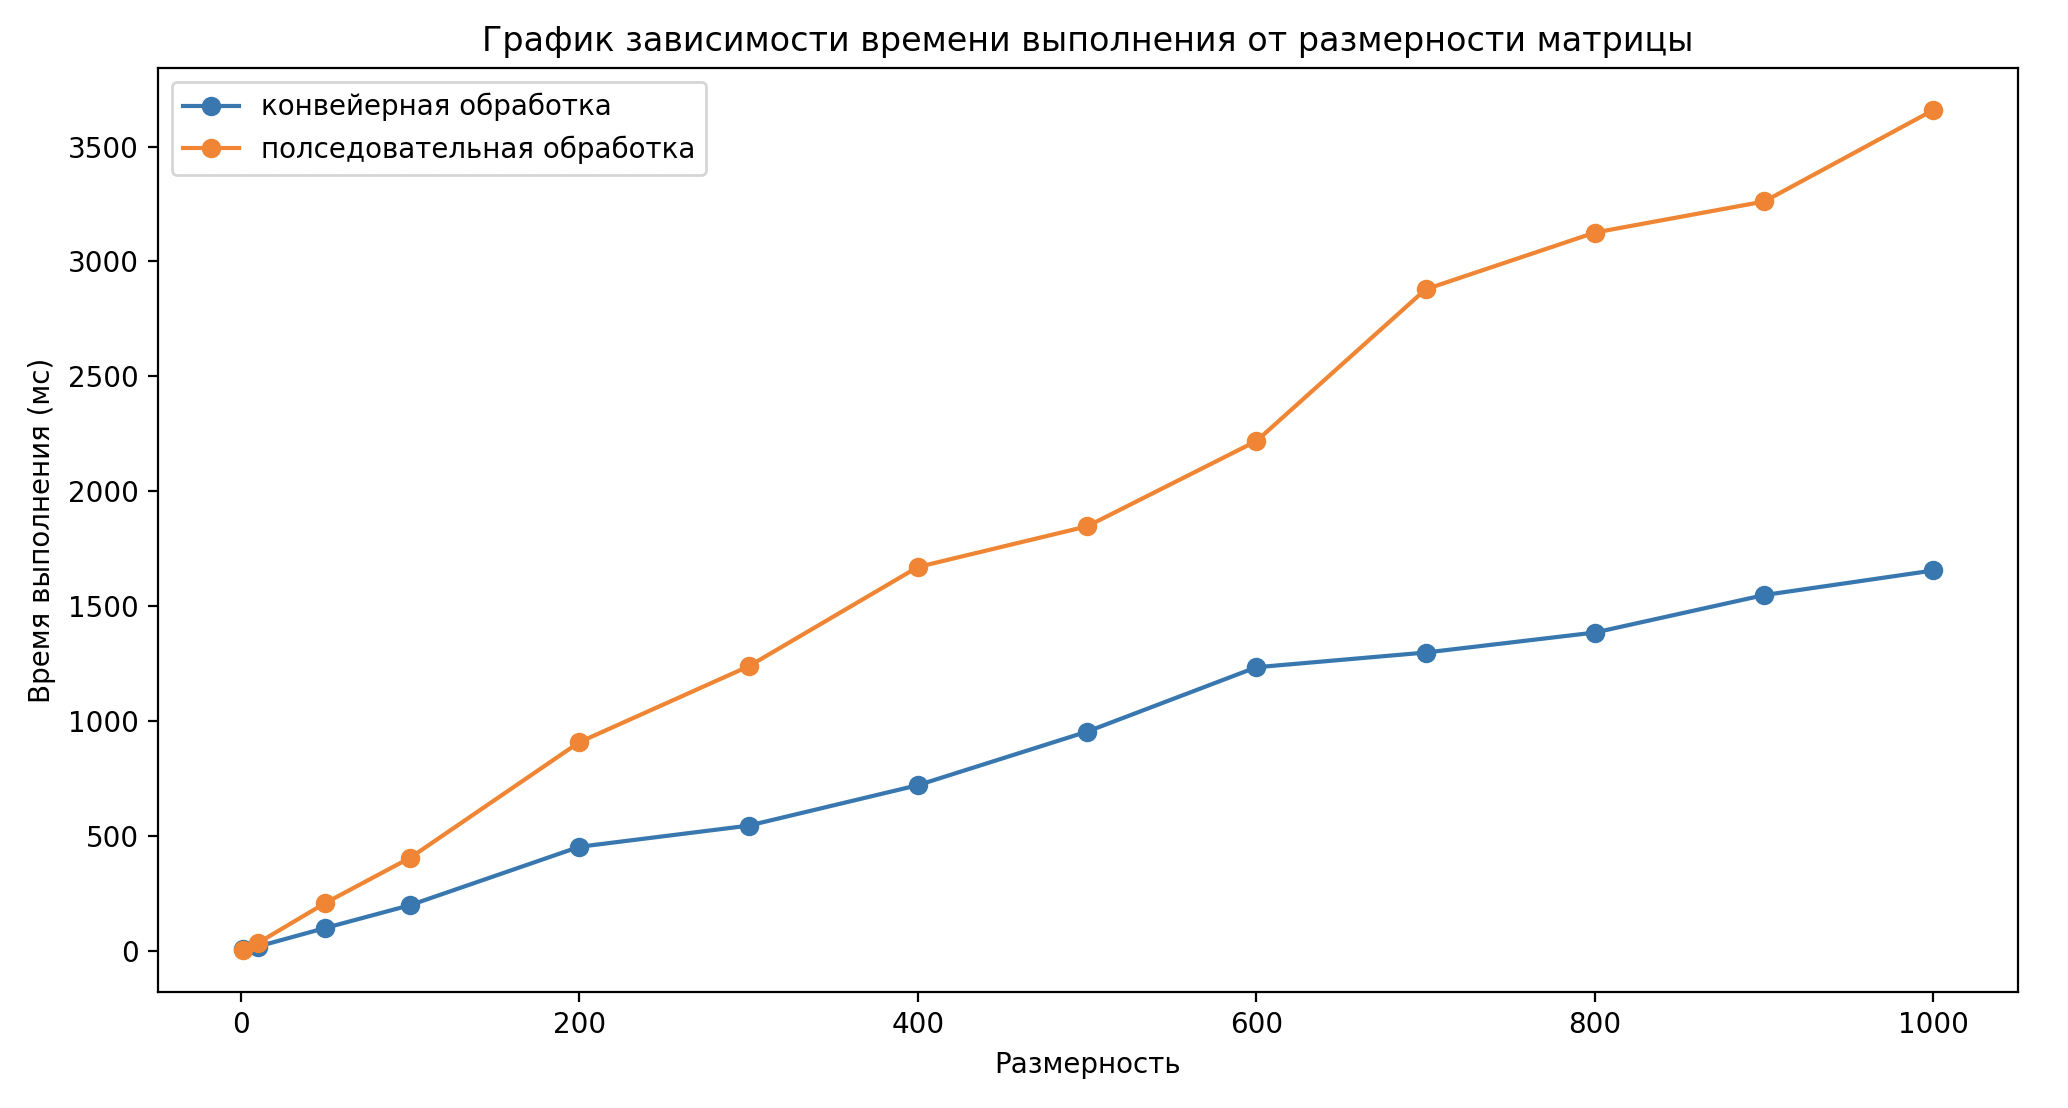
\includegraphics[width=1\linewidth]{img/graph.png}
    \caption{График зависимости времени выполнения работы от размерности матрицы}
    \label{fig:graph}
\end{figure}

\clearpage
\section{Вывод}
Таким образом, для ускорения обработки объектов, которая состоит из нескольких этапов,
необходимо использовать конвейерную обработку.
